\subsection{Functions of Multiple Variables}

\subsubsection{Classification of 3D Surfaces}
So far, we have only been working in the 2D plane with functions of 2 variables: $y=f(x)$. We can extend the same ideas to higher dimensions: A function $z=f(x,y)$ will form a surface in 3 dimensions and a function $w=f(x,y,z)$ will span 4 dimensions. While we are still able to analyze the behaviors of higher dimensional systems, we will often stick to functions of 3 variables for the sake of visualization.\\

As with 2D, there are a few common functions that you should recognize and be able to plot.
\begin{enumerate}
    \item Planes\\
    These are of the form $z=ax+by+c$ (as seen in a previous section)\\
    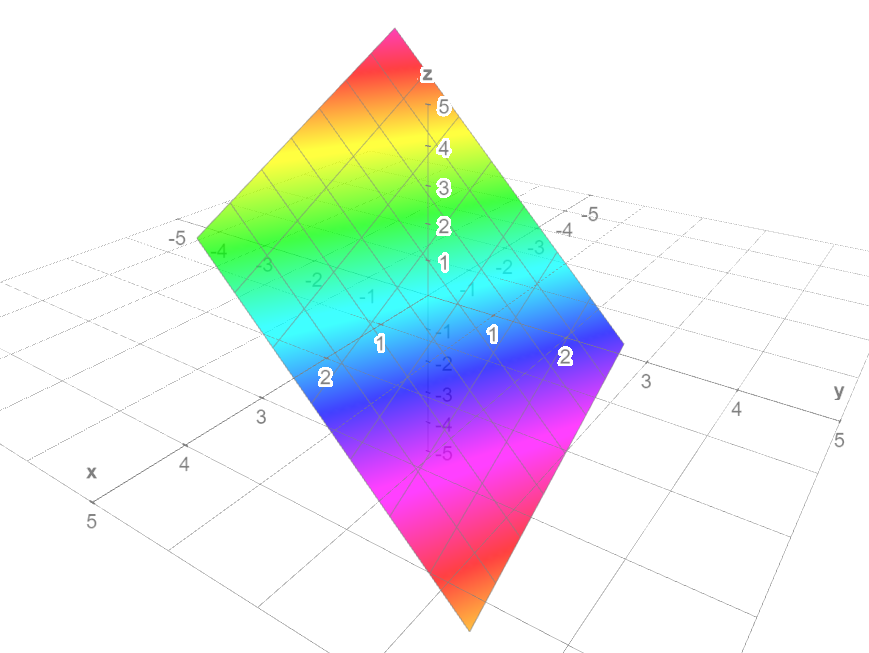
\includegraphics[scale=0.5]{Images/Math217Pictures/planeGraph.png}
    \item Spheres\\
    These are of the form $x^2+y^2+z^2=r^2$ (similar to a circle in 2D)\\
    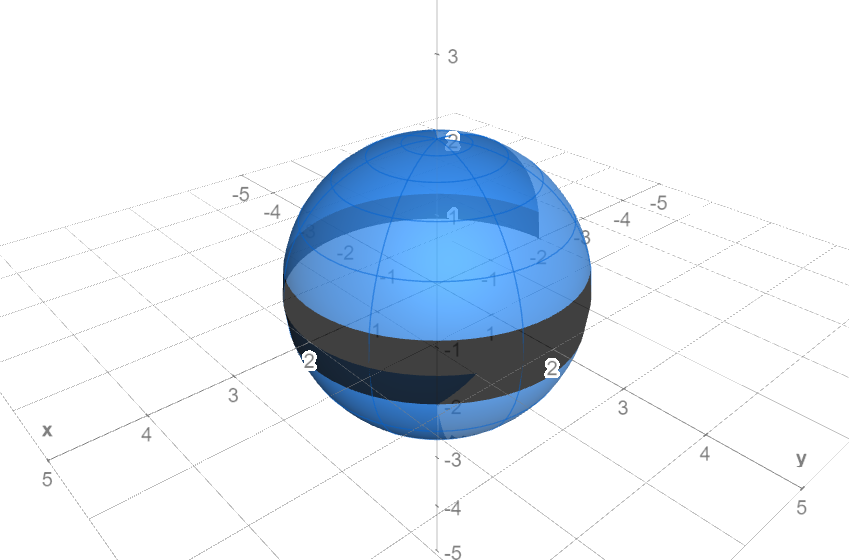
\includegraphics[scale=0.5]{Images/Math217Pictures/sphereGraph.png}
    \item Cylinders\\
    These are of the form $x^2+y^2=1$. Note that this is a function defined in terms of only $x$ and $y$ so it will be the same for all $z$.\\
    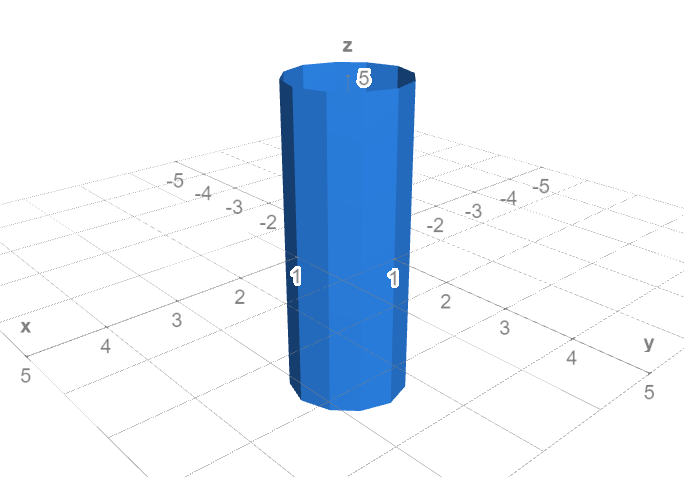
\includegraphics[scale=0.4]{Images/Math217Pictures/cylinderGraph.png}
    \item Cones\\
    These are of the form $z=\sqrt{x^2+y^2}$ for a one-sided cone and $z^2=x^2+y^2$ for a two-sided cone.\\
    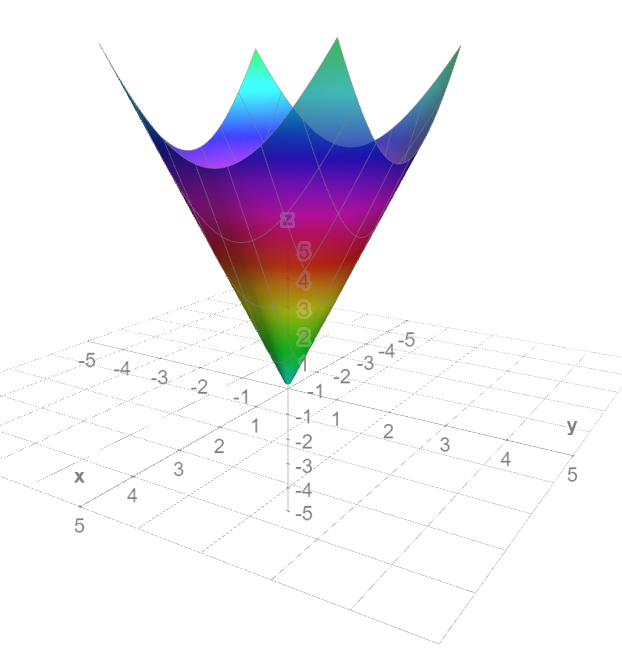
\includegraphics[scale=0.4]{Images/Math217Pictures/coneGraph.png}
    \item Paraboloids\\
    These are of the form $z=x^2+y^2$\\
    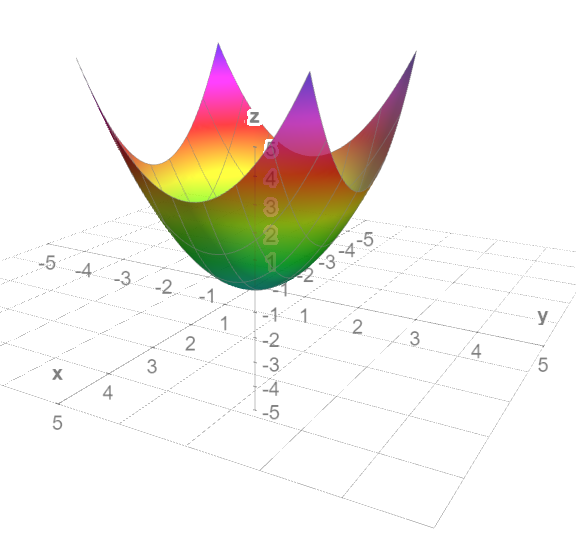
\includegraphics[scale=0.6]{Images/Math217Pictures/parabaloidGraph.png}
    \item Saddles\\
    These are of the form $z=x^2-y^2$\\
    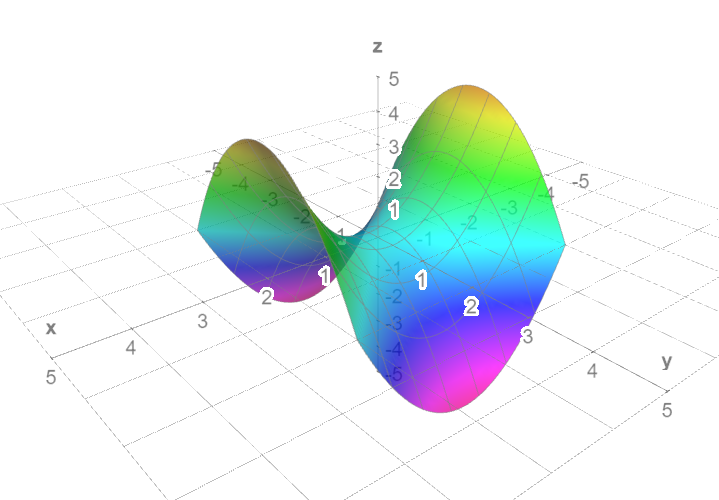
\includegraphics[scale=0.5]{Images/Math217Pictures/saddleGraph.png}
\end{enumerate}
There are many more functions not mentioned such as ellipsoids, hyperboloids, and parabolic cylinders but this should be enough to begin to get an idea of what 3D functions look like.

\subsubsection{Sketching Surfaces}
Sketching surfaces in 3D is often trickier than in 2D but there are a few useful tricks to get an idea what the surface looks like.\\
One of the most useful ones is level curves. This is where if we have a function $z=f(x,y)$, we set $z$ to be a constant and draw the curve on the xy-plane for varying $z$ (in 2D these are called contour plots).\\
In short, a contour plot is an overlay of lines of $f(x,y)=k$ plotted on the xy-plane. The rate of greatest change (the gradient) is always perpundicular to the contour lines.\\
Similarly, a level surface is the overlay of surfaces of $f(x,y,z)=k$ plotted in 3-space (or higher).
Ex: $z=x^2+4y^2-2x+2$\\
\centerline{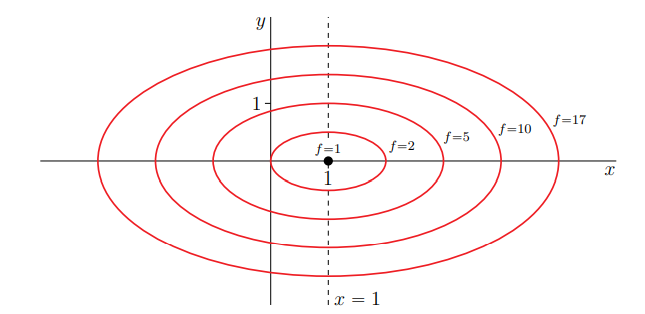
\includegraphics[scale=0.8]{Images/Math217Pictures/contourPlot.png}}
This becomes increasingly useful for visualizing functions in 4 dimensions as we can define their level curves as 3D functions.\\
Ex: $F=x^2+y^2+z^2$\\
\centerline{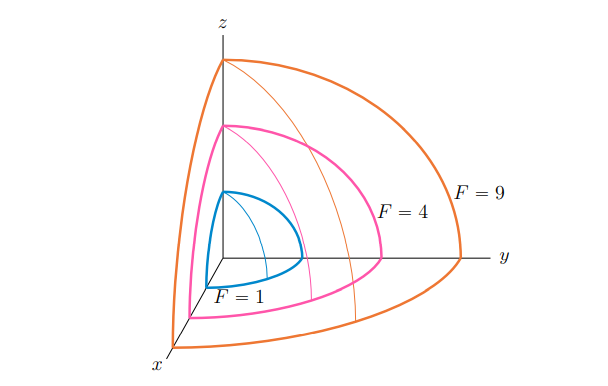
\includegraphics[scale=0.8]{Images/Math217Pictures/levelCurves.png}}
Sometimes it can be useful to sketch contour plots in multiple planes as it may be easier or give different perspectives.\\
Other useful tricks in sketching curves that will be seen later may be to take the gradient (as it gives a vector field normal to the level curves at all points) or to find the critical points of the function.
